% The ATLAS calorimeter system~\cite{atlas_calorimeter_tdr}, shown in Figure~\ref{fig:atlas_calorimeter}, is the next major sub-system of the ATLAS detector, and is designed to measure the energy of all particles, excluding muons and neutrinos, that traverse it in the pseudorapidity range of $|\eta| < 4.9$\@. The calorimeter system is split into three sub-detectors: the Electromagnetic Calorimeter (ECal), the Hadronic Calorimeter (HCal), and the Forward Calorimeter (FCal). 

% The ECal is the innermost layer of the calorimeter system and surrounds the ID\@. It consists of a barrel section and two end-caps, and its primary function is to measure the energy of electromagnetic particles, such as electrons and photons. The HCal surrounds the ECal and is designed to measure energy deposited by hadrons, jets, taus and missing transverse energy (\met). Finally, the FCal, is located in the very forward region between the hadronic end-caps and the beam pipe. The FCal includes both electromagnetic and hadronic components and extends the detector acceptance in the high $|\eta|$ region.

% Particles deposit energy in the calorimeter in different ways depending on their type. Electrons, for example, lose energy primarily via bremsstrahlung radiation, while photons primarily lose their energy via pair production when passing through the passive material in the ECal. These interactions occur over a characteristic distance known as the radiation length \radlength, which is defined as the average distance over which a high energy particle loses all but 1/$e$ (37\%) of its energy. The radiation length depends on the material and is given empirically by equation~\ref{eq:rad_length}:

% \begin{equation}
%     \centering
%     X_{0} = 716.4 \ \mathrm{g \ cm^{-2} \ \frac{A}{Z (Z+1) \ln{\frac{287}{\sqrt{Z}}}}}
%     \label{eq:rad_length}
% \end{equation}

% \noindent{}where $A$ is the atomic mass number and $Z$ is the atomic number of the absorber material. A small radiation length is desirable in the ECal to ensure that the electromagnetic showers are contained within this detector.

% Hadrons, in contrast, lose energy primarily through inelastic interactions with nuclei in the absorber material. These interactions produce secondary particles, leading to a hadronic shower. The amount of particles remaining after traveling a distance $x$ through a material is given by equation~\ref{eq:hadronic_num_remaining}:

% \begin{equation}
%     \centering
%     N(x) = N_{0} e^{-\frac{x}{\lambda}}
%     \label{eq:hadronic_num_remaining}
% \end{equation}

% \noindent{}where $N_{0}$ is the initial number incoming particles, and $\lambda$ is the nuclear interaction length, defined as:

% \begin{equation}
%     \centering
%     \lambda_{a} = 35 \ \mathrm{g \ cm^{-2}} \ A^{\frac{1}{3}}
%     \label{eq:absorption_length}
% \end{equation}

% \noindent{}This length is the average distance a hadron travels before under-going a nuclear interaction. Lighter materials with small $A$ have smaller interaction lengths, resulting in more interactions, and therefore are more suitable for the HCal\@.

% The ATLAS calorimeters use different technologies depending on their purpose. The ECal and the end-cap regions of the HCal and FCal are based on liquid argon (LAr) technology. The central barrel of the HCal uses a scintillating Tile calorimeter, where the absorber is steel, and the active material is a plastic scintillator. All of the calorimeters are sampling calorimeters, meaning they are composed of alternating layers of absorber and active materials.

% \begin{figure}
%     \centering
%     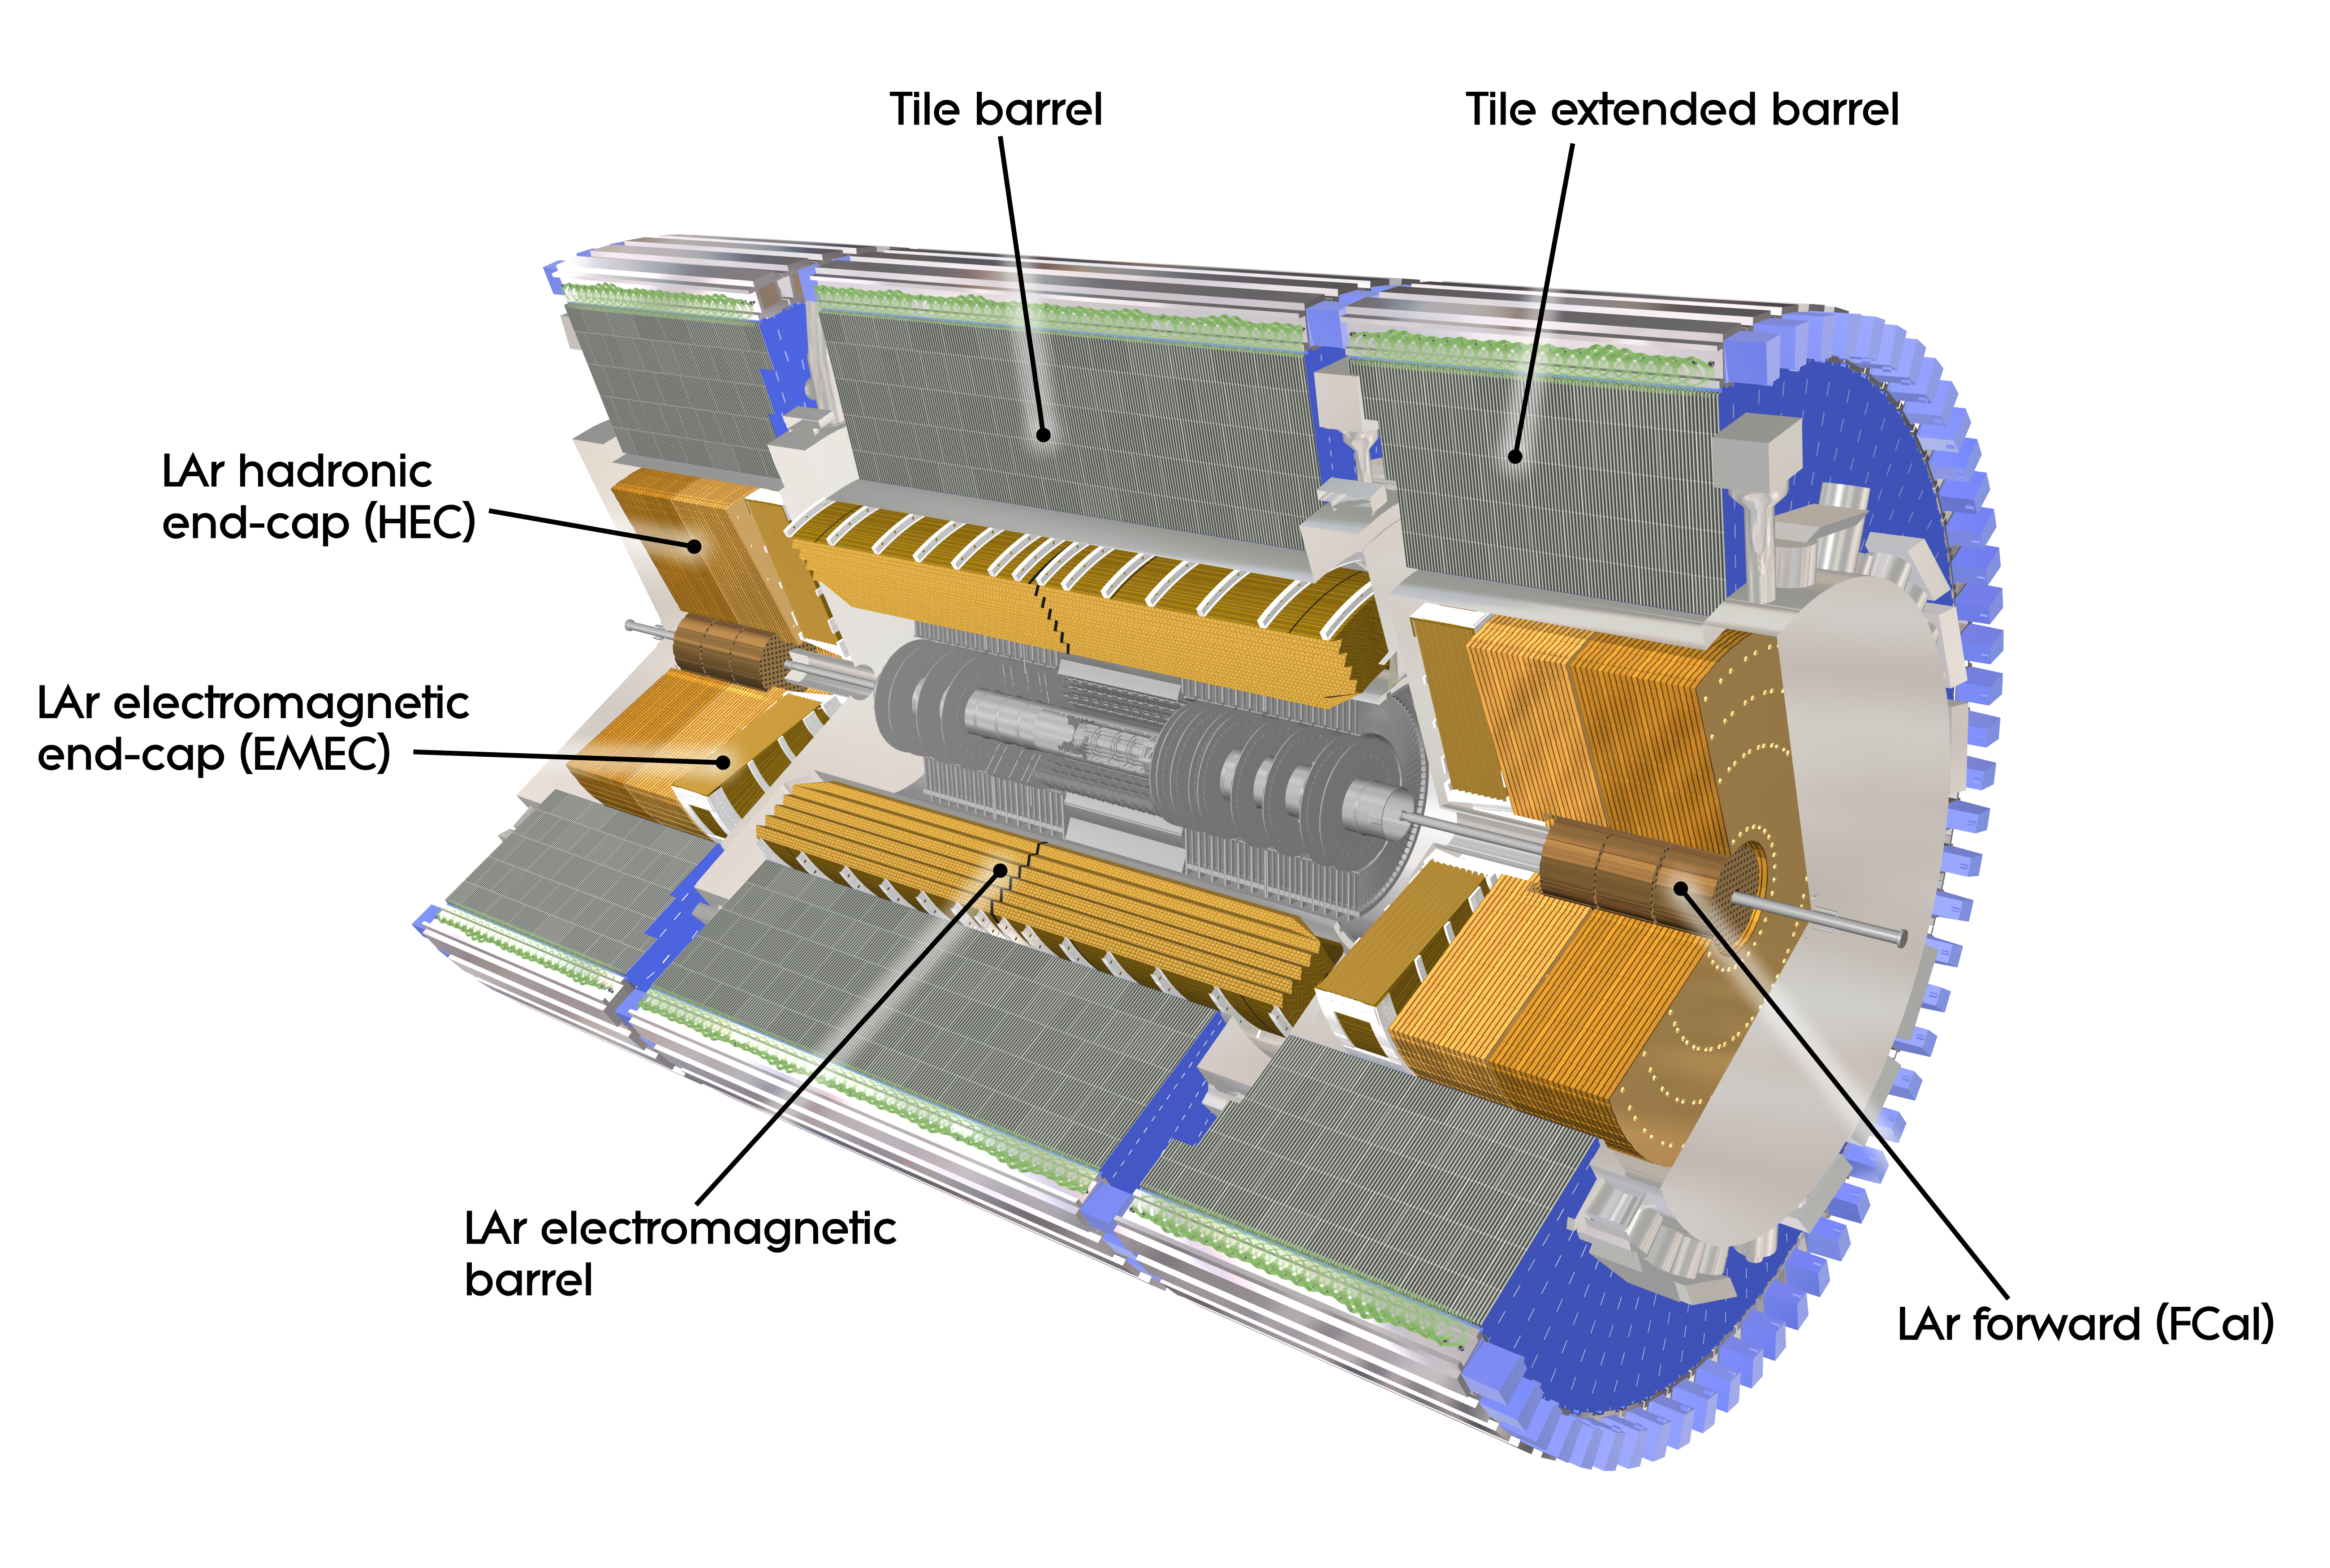
\includegraphics[width=0.8\textwidth]{figures/atlas/atlas_calorimeter.jpg}
%     \caption{Cut away view of the ATLAS calorimeter system is depicted. The first layer of the calorimeter is the EM calorimeter, surrounded by the hadronic calorimeter. Taken from~\cite{atlas_tile_calorimeter}}\label{fig:atlas_calorimeter}
% \end{figure}


%%%%%%%%%%%%%%%% Revision

The ATLAS calorimeter system~\cite{atlas_calorimeter_tdr} measures the energy of all particles except muons and neutrinos within the pseudorapidity of $|\eta| < 4.9$\@. It consists of three sub-detectors: the Electromagnetic Calorimeter (ECal), the Hadronic Calorimeter (HCal), and the Forward Calorimeter (FCal). 

The ECal surrounds the ID and measures the energy of electrons and photons and consists of a barrel and two end-caps. The HCal surrounds the ECal and measures energy deposited by hadrons, jets, taus and missing transverse energy (\met). The FCal is located in the very forward region between the hadronic end-caps and the beam pipe extending the $|\eta|$ region and has both EM and hadronic components. 

Electrons primarily lose energy via bremsstrahlung radiation, while photons primarily lose their energy via pair production when passing through the passive material in the ECal. These interactions occur over a characteristic radiation length \radlength, defined as the average distance in which high energy particle loses all but 1/$e$ (37\%) of its energy. The \radlength{} depends on the material and is given empirically by

\begin{equation}
    \centering
    X_{0} = 716.4 \ \mathrm{g \ cm^{-2} \ \frac{A}{Z (Z+1) \ln{\frac{287}{\sqrt{Z}}}}}
    \label{eq:rad_length}
\end{equation}

\noindent{}where $A$ is the atomic mass number and $Z$ the atomic number of the absorber material. A small radiation length is ideal for the ECal to ensure that the EM shower is contained.

Hadrons primarily lose energy through inelastic interactions with nuclei in the absorber material. These interactions produce secondary particles resulting in a hadronic shower. The amount of particles remaining after traveling a distance $x$ is given by $N(x) = N_{0} e^{-\frac{x}{\lambda}}$ where $N_{0}$ is the initial number incoming particles, and $\lambda$ is the nuclear interaction length, defined as:

\begin{equation}
    \centering
    \lambda_{a} = 35 \ \mathrm{g \ cm^{-2}} \ A^{\frac{1}{3}}
    \label{eq:absorption_length}
\end{equation}

\noindent{} where $\lambda$ represents the average distance a hadron travels before under going a nuclear interaction. Light materials with small $A$ have more interactions and therefore are more suitable for the HCal\@.

The calorimeters use different technologies depending on their purpose. The ECal, HCal end-caps, and FCal use liquid argon (LAr) while the center barrel of the HCal uses steel-scintillator Tile. All calorimeters are sampling calorimeters since they are composed of alternating layers of absorber and active materials.

\begin{figure}
    \centering
    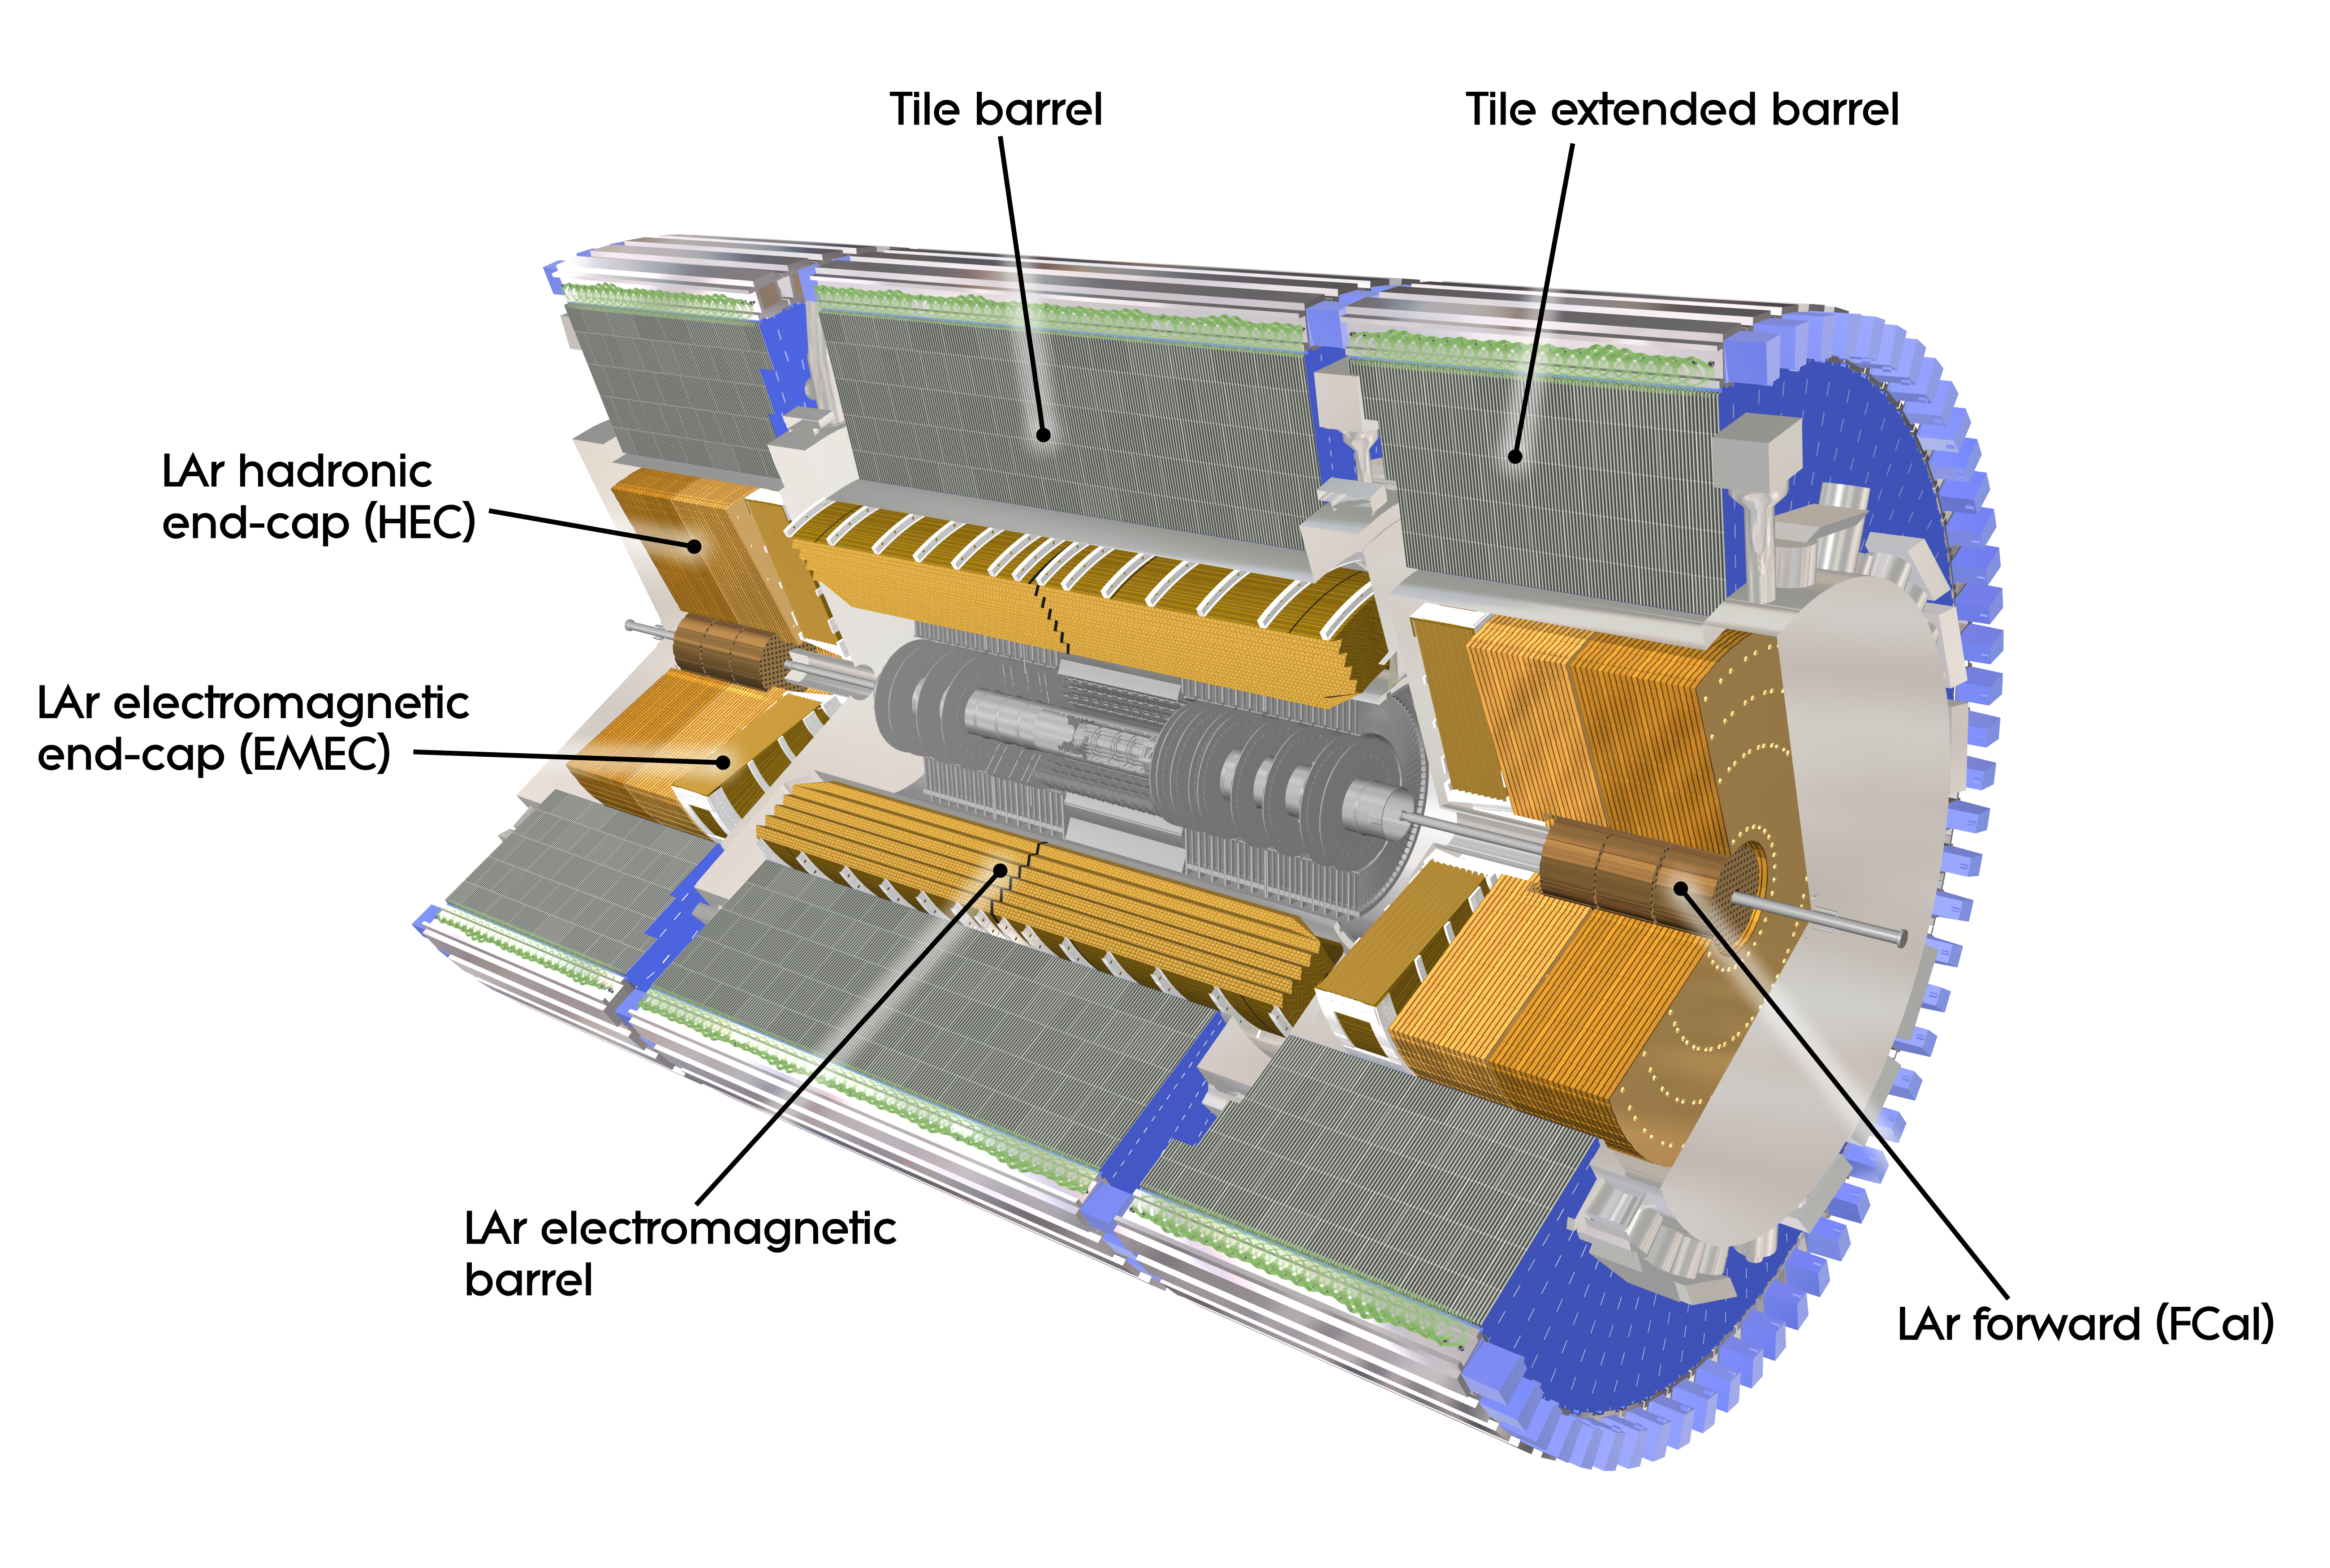
\includegraphics[width=0.8\textwidth]{figures/atlas/atlas_calorimeter.jpg}
    \caption{Cut away view of the ATLAS calorimeter system is depicted. The first layer of the calorimeter is the EM calorimeter, surrounded by the hadronic calorimeter. Taken from~\cite{atlas_tile_calorimeter}}\label{fig:atlas_calorimeter}
\end{figure}